
\subsection{Problem Formulation and Main Results}

%Suppose we have $t$ labeled regression tasks. %where $t$ is a fixed value that does not grow with the feature dimension $p$.
%For each task $k$ from $1$ to $t$, we have $n_k$ samples $x_1, x_2, \dots, x_{n_k}$ that are all $p$-dimensional feature vectors with real-valued labels $y_1, y_2, \dots, y_{n_k}$.
%Without loss of generality, we focus on predicting the $t$-th task and refer the $t$-th task as the target.
%We refer to task $1$ to task $t-1$ as source tasks.
%We assume that the labels of each task $k$ satisfy the linear model with unknown parameters $\beta_k\in\real^p$, that is,
%	\[ y_i = x_i^{\top}\beta_k + e_i, \text{ for all } 1 \le i \le n_k, \]
%where $e_i$ denotes random noise with mean zero and variance $\sigma^2$.
%To write the above notations more succiently, let $X_k \in \real^{n_k \times p}$ denote the covariates that consists of a feature vector in every row.
%Let
%	\be\label{model_YvsX} Y^{(k)} = X^{(k)} \beta_k + \varepsilon_k, \text{ for all } 1\le k \le t \ee denote the label vector of task $k$ and $\varepsilon_k$ denote an i.i.d. random vector with mean zero and variance $\sigma^2$.
%Following \citet{HMRT19} and \citet{BLLT20},
%In the high-dimensional linear regression setting (e.g. ), the features of the $k$-th task, denoted by $X_k\in\real^{n_i\times p}$, consist of $n_k$ feature vectors given by $x_1, x_2, \dots, x_{n_k}$.
%we assume that for each task $k$ from $1$ to $t$, each feature vector $x_i = \Sigma^{1/2}_k z_i$ for $i = 1, \dots, n_k$, where $z_i\in\real^p$ is an i.i.d. random vector with  mean zero and unit variance.
%Recall that $\Sigma_k$ is the population covariance matrix task $k$'s feature vectors.
%Let $\Sigma_k = U_k D_k U_k^{\top}$ denote the singular value decomposition of $\Sigma_k$.
%We denote $\Sigma_k = U_k D_k^{1/2}$ as the square root of $\Sigma_k$.
%The sample size of task $k$, given by $n_k$, is equal to $\rho_k\cdot p$ for a fixed value $\rho_k$ that does not grow with feature dimension $p$.
%This setting is also known as the high-dimensional linear regression setting in the literature.
%There are two motivations for studying the high-dimensional linear regression setting for multi-task learning.
%First, this setting captures salient properties of modern large-scale datasets, where the sample sizes are usually on the order of tens to hundreds of the number of features \cite{sur2019modern}.
%Second, as we will see soon in Section \ref{sec_general}, we can derive precise asymptotics of the generalization error that scale with properties of the task data such as sample sizes.
%The labels $Y_k = X_k \beta_k + \varepsilon_k$, where $\beta_k$ denotes the linear model parameters and $\varepsilon_k$ denotes i.i.d. noise with mean zero and variance $\sigma^2$.
%Recall that we have $t$ labeled training datasets, denoted by $(X_1, Y_1), (X_2, Y_2), \dots, (X_t, Y_t)$, where $X_i\in\real^{n_i\times p}$ and $Y_i\in\real^{n_i}$ for $1\le i\le t$.
%Following \cite{HMRT19,BLLT20}, we assume that for each task $i = 1,2,\dots,t$,  every feature vector is generated as $x = \Sigma_i^{1/2} z$, where $z\in\real^p$ is a random vector with i.i.d. entries of mean zero and unit variance and $\Sigma_i\in\real^{p\times p}$ is a positive semidefinite matrix.
%Without loss of generality, let the $t$-th task be the target task.

Regression analysis is arguably one of the most fundamental methods in statistics and machine learning.
In many applications of multi-task learning, the amount of labeled data from each dataset is usually insufficient for learning a single task.
For example, this is the case if a dataset's sample size is only a small constant times the dimension of the feature vectors \cite{GLUE}.
In this paper, we consider multi-task learning in a high-dimensional linear regression setting.
We assume that there are multiple datasets that all follow a (potentially different) linear model.
In each dataset, we assume the feature vector $x = {\Sigma}^{1/2} z$, where $z \in \real^p$ has i.i.d entries with mean zero, unit variance, and covariance $\Sigma \in\real^{p \times p}$ that is deterministic and positive semidefinite.
We are mainly interested in the \textit{high-dimensional} setting, where each dataset's sample size and the feature dimension grow linearly at a fixed ratio.
This setting is particularly challenging, but is crucial for understanding how datasets' properties such as their sample sizes impact generalization performance.

We study a hard parameter sharing architecture to learn jointly from multiple datasets.
In this architecture, there is a shared feature representation layer $B\in\real^{p\times r}$ for all tasks, and a task-specific output layer $A_i \in \real^r$ for every task $i$ to $t$.
Suppose we have $t$ datasets.
For each task $i = 1, 2, \dots, t$, let $n_i$ denote its sample size, $X^{(i)} \in \real^{n_i \times p}$ denote its feature covariates, and $Y^{(i)} \in \real^{n_i}$ denote all the labels.
%The width of $B$, denoted by $r$, plays an important role in regularization.
%As observed in Proposition 1 of \citet{WZR20}, if $r \ge t$, there is no regularization effect.
%Hence, we assume that $r < t$ in our study.
%For example, when there are only two tasks, $r = 1$ and $B$ reduces to a vector whereas $W_1, W_2$ become scalars.
Let $A = [A_1, A_2, \dots, A_t] \in \real^{r \times t}$.
We study the following optimization objective.
%	\item Separate each dataset $(X_i, Y_i)$ randomly into a training set $(X_i^{tr}, Y_i^{tr})$ and a validation set $(X_i^{val}, Y_i^{val})$.
%	The size of each set is described below.
%	\item Learn the shared layer $B$: minimize the training loss over $B$ and $W_1, \dots, W_t$, leading to a local minimum of $B$ that depends on $W_1, \dots, W_t$, denoted by $\hat{B} = \hat{B}(W_1, \dots, W_t)$.
\begin{align}\label{eq_mtl}
			f(A, B) = \sum_{i=1}^t \norm{X^{(i)} B A_i - Y^{(i)}}^2.
\end{align}
Given a solution $\hat{A}, \hat{B}$ from the above optimization, let $\hat{\beta}_i^{\MTL} = \hat{B} \hat{A}_i$ denote the hard parameter sharing (HPS) estimator for task $i$.
The important questions here are:
(i) how well does the estimator work? In particular, how does the performance of the estimator scale with sample size?
(ii) for datasets with different sample sizes and covariate shifts, how do they impact the estimator?


%	\item Learn the output layers $W_1, W_2, \dots, W_t$: set $B = \hat{B}$ and minimize the training loss over $W_1, W_2, \dots, W_t$.
%		{\begin{align}\label{eq_mtl_eval}
%			g(W_1, \dots, W_t) = \sum_{k=1}^t \norm{X_k \hat{B} W_k - Y_k}^2.
%		\end{align}}
%\end{enumerate}
%Let $\hat{\beta}_t^{\MTL}$ denote the multi-task learning estimator obtained from the procedure above.
%By contrast, let $\hat{\beta}_t^{\STL} = (X_t^{\top}X_t)^{-1}X_t^{\top}{Y_t}$ denote the single-task learning estimator. % denoted by $L(\hat{\beta}_t^{\STL})$.
%where $B\in\real^{p\times r}$ and $W_k\in\real^r$ for every $1\le k\le t$.
%Following , we assume that $r < t$, because otherwise minimizing $f(\cdot)$ could result in $BW_i$ being the single-task optimum.
%\smallskip
%\noindent\textit{Remark.}
%In general, the multi-task learning objective $f(\cdot)$ is non-convex with respect to $B$ and $W_1, \dots, W_t$.
%Therefore, we first minimize $B$ in equation \eqref{eq_mtl} and then minimize $W_k$ given $B$ in equation \eqref{eq_mtl_eval}.
%For our results later in Section \ref{sec_general} and \ref{sec_special}, we will identify tractable cases and provide guarantees to the above procedure.
%\paragraph{Problem statement.}
%We focus on predicting a particular task, say the $t$-th task, without loss of generality.
%For an estimator $\hat{\beta}$ of the target task model $\beta_t$, we define the prediction loss of the estimator $\hat{\beta}$ as
%	{\begin{align}\label{eq1_prediction_loss}
%		\te(\hat{\beta}) = \exarg{x = \Sigma_t^{1/2} z}{({x}^{\top}\hat{\beta} - {x}^{\top}\beta_t)^2}
%		= \bignorm{\Sigma_t^{1/2} (\hat{\beta} - \beta_t)}^2,
%	\end{align}}%
%where $x = \Sigma_t^{1/2} z$ denotes a random feature vector with covariance $\Sigma_t$.
%In the above equation, $x^{\top}\beta_t$ is the true label of $x$.
%= (\hat{\beta} - \beta_t)^{\top}\Sigma_t(\hat{\beta} - \beta_t)
%We say that the source tasks provide a \textit{positive transfer} to the target task if the prediction loss of the MTL estimator is lower than that of the STL estimator, that is, if
%	\[ L(\hat{\beta}_t^{\MTL}) > L(\hat{\beta}_t^{\STL}). \]
%On the other hand, we say that the source tasks provide a \textit{negative transfer} to the target task if $L(\hat{\beta}_t^{\MTL}) < L(\hat{\beta}_t^{\STL})$.
%Our goal is to study when the source tasks provide a positive transfer to the target task.
%More specifically, we study how varying properties of task data including task similarity, sample ratio, and covariate shift affects information transfer in multi-task learning.

%We begin by defining our problem setup including the multi-task estimator we study.
%Then, we describe the bias-variance tradeoff of the multi-task estimator and connect the bias and variance of the estimator to \textit{task similarity}, \textit{sample size}, and \textit{covariate shift}.
%Finally, we show a tight concentration bound for the bias and variance quantities using random matrix theory.

%\subsection{Problem Formulation}

%In the worst case, the optimization objective \eqref{eq_mtl} is non-convex in $A$ and $B$ (e.g. matrix completion is a special case for suitably designed $X^{(i)}, Y^{(i)}$).
%Therefore, we work in cases where a global and/or local minimum characterization is possible

\paragraph{Main results.}
Our first result (Theorem \ref{thm_many_tasks}) applies to the multi-label prediction setting where all datasets have the same features, and we want to make multiple predictions (e.g. \cite{hsu2009multi}).
We analyze the global minimum of $f(A, B)$, and provide a sharp generalization bound for its (out-of-sample) prediction loss for any task.
This is a tractable special case of the general problem because in the worst case, $f(A, B)$ is non-convex in $A$ and $B$ (e.g. matrix completion is a special case for suitably designed $X^{(i)}, Y^{(i)}$).
We show that the prediction loss of hard parameter sharing admits a clean bias-variance decomposition.
Our results imply that hard parameter sharing helps by reducing variance compared to single-task learning, but hurts by increasing bias.
Our second result (Theorem \ref{thm_main_RMT}) applies to two tasks with arbitrarily different sample sizes and covariance matrices.
We analyze the local minimum of $f(A, B)$, and provide a sharp generalization bound for its prediction loss for both tasks.
Despite its simplicity, we show several rich phenomena by varying sample sizes and covariate shifts in this setting.
See Figure \ref{fig_intro_sample_size} for an illustration.

\begin{figure}[!t]
	\begin{subfigure}[b]{0.5\textwidth}
		\centering
		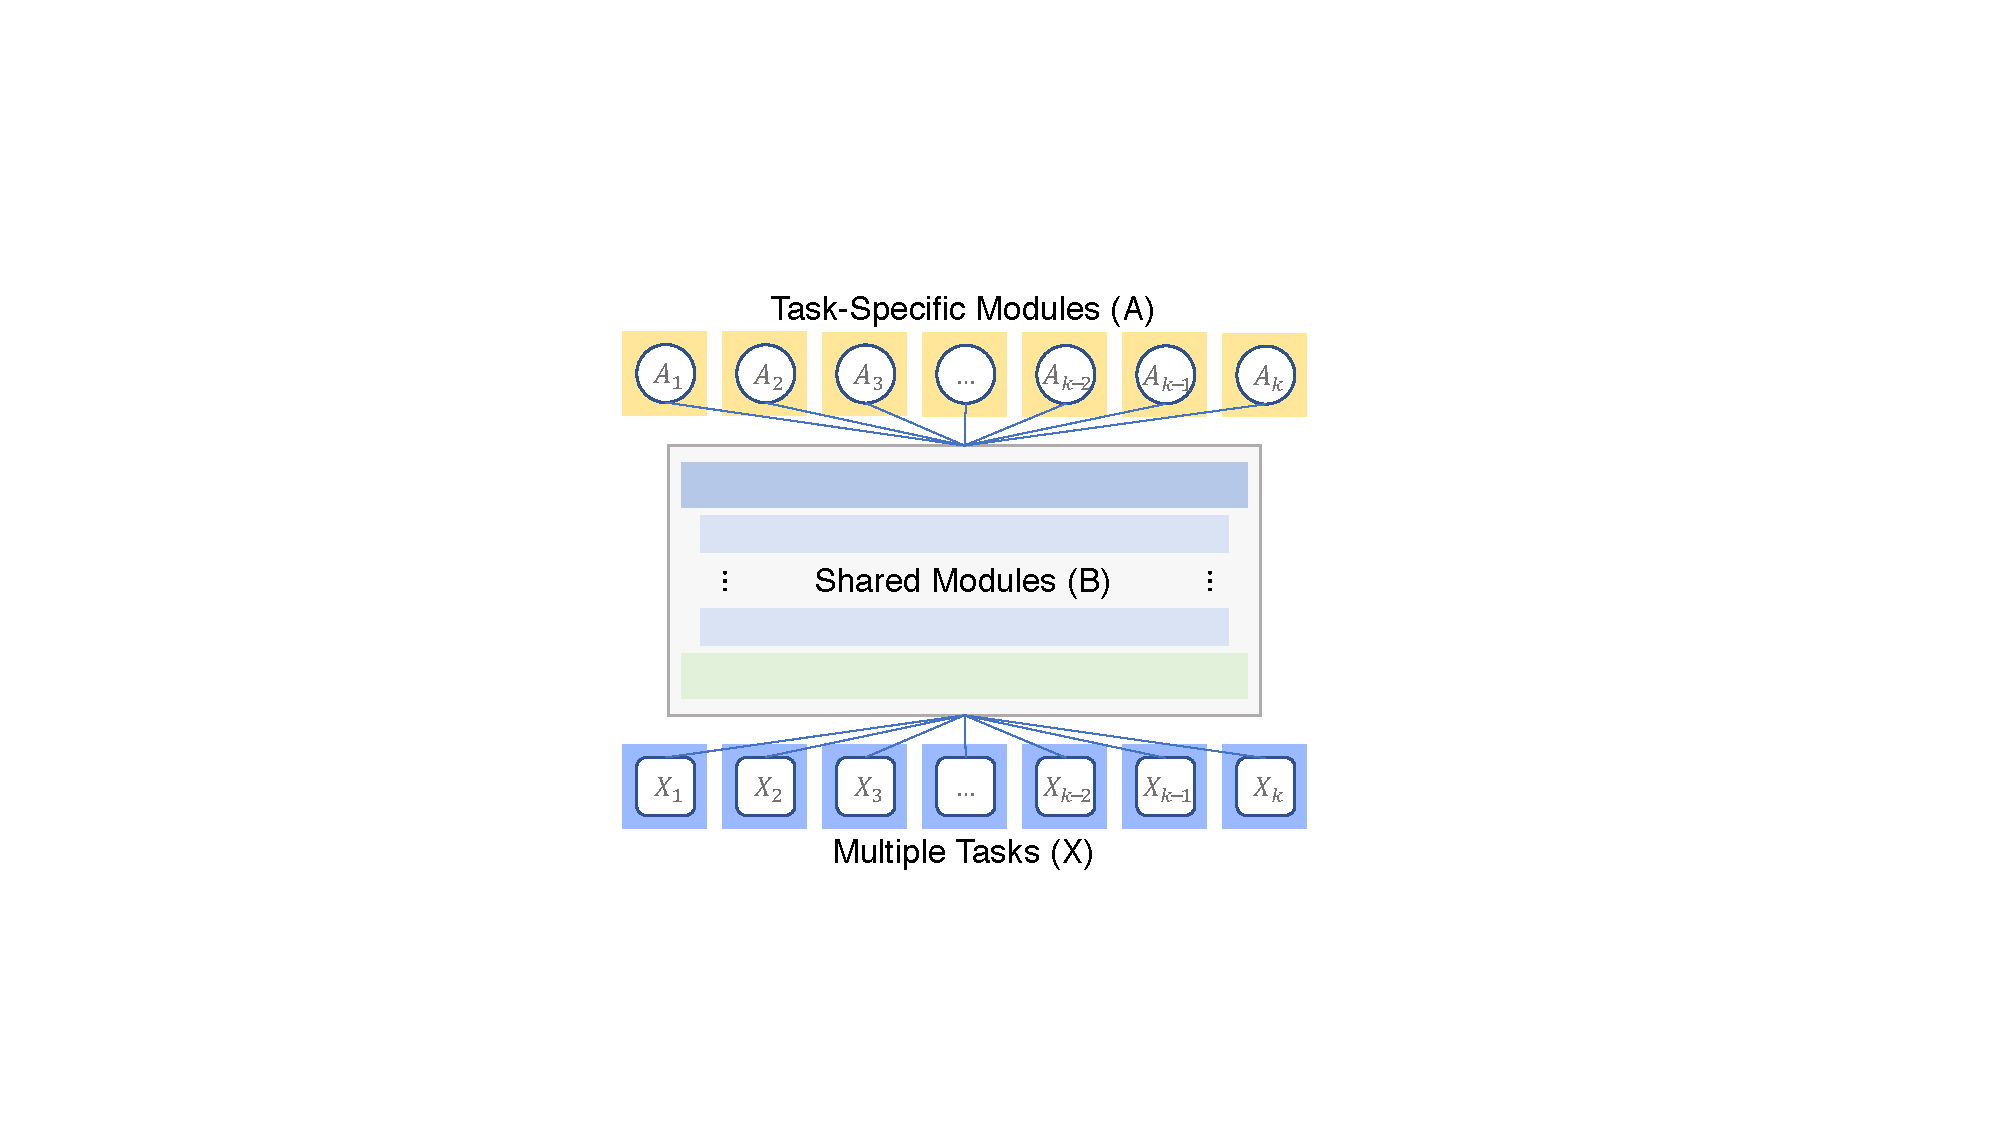
\includegraphics[width=0.65\textwidth]{figures/mtl_model.pdf}
		\caption{A hard parameter sharing architecture}
	\end{subfigure}\hfill
	\begin{subfigure}[b]{0.5\textwidth}
		\centering
		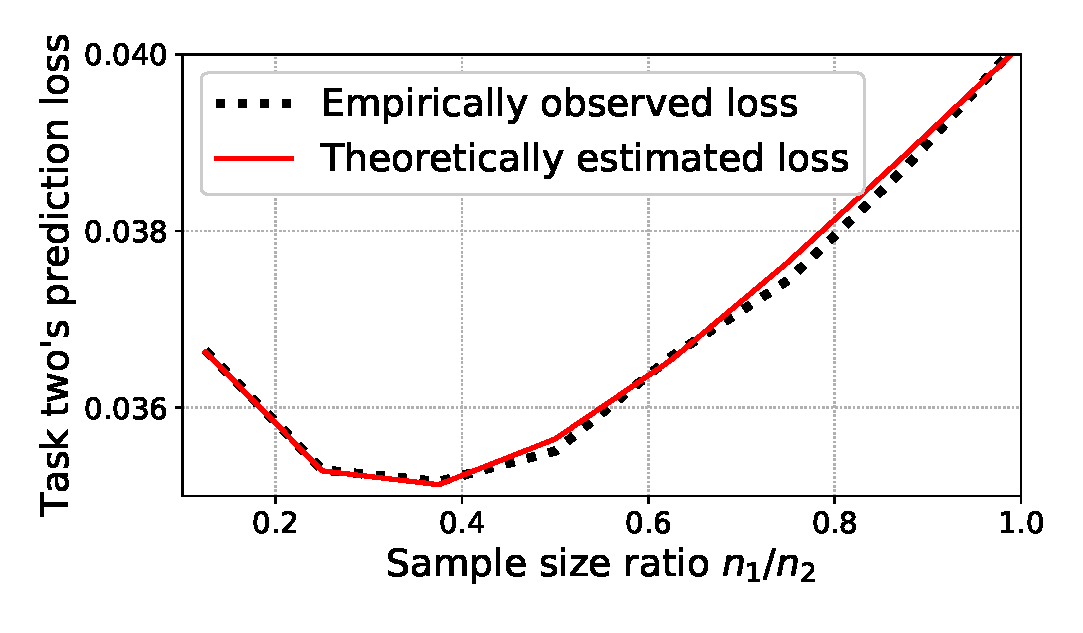
\includegraphics[width=0.9\textwidth]{figures/sample_ratio_c2_400.eps}
		\caption{Varying sample size ratio}
		\label{fig_intro_sample_size}
	\end{subfigure}
	\caption{An illustrative example of our result:
	Consider the prediction loss of hard parameter sharing (left) for task two, given two linear regression tasks.
	Increasing task one's sample size helps reduce task two's prediction loss initially, but increases afterwards. Our result provides an estimated loss (solid line) that matches the empirical loss (dotted line) accurately. This phenomenon occurs due to different bias-variance tradeoffs as the sample size ratio increases.
	See Section \ref{sec_simulation} for the precise setting.}
	\label{fig_intro_sample_size}
\end{figure}

As a consequence of our concrete and precise loss estimates, we observe qualitative properties of hard parameter sharing for varying datasets' properties.
\begin{enumerate}
	\item \textit{Sample efficiency (Example \ref{ex_same_cov})}:
	One advantage of combining multiple datasets is that the requirement for labeled data reduces compared to STL, a phenomenon that is empirically observed in Taskonomy \cite{ZSSGM18}.
	Our results further show that HPS's sample efficiency depends on task-specific variance vs. noise variance. It is generally high when the noise variance is large compared to model-specific variance across tasks.
	\item \textit{Sample size ratio (Example \ref{ex_sample_ratio})}: Increasing one task's sample size does not always help reduce another task's loss. We find in a simplified setting that depending on how much bias increases, the task loss either decreases first before increasing afterwards, or decreases monotinically. These two trends result from different tradeoffs between increasing bias and decreasing variance.
	\item \textit{Covariate shift (Example \ref{ex_covshift})}: In addition to sample sizes, variance also scales with the covariate shift between different datasets. For high sample size ratio, variance is smallest when there is no covariate shift. Counterintuitively, for low sample size ratio, having covariate shift reduces variance through a complementary spectrum.
\end{enumerate}

%First, we develop tight bounds for the bias and variance of the multi-task estimator for two tasks by applying recent development in random matrix theory \cite{erdos2017dynamical,isotropic,Anisotropic}.
%We observe that the variance of the multi-task estimator is \textit{always smaller} than single-task learning, because of added source task samples.
%On the other hand, the bias of the multi-task estimator is \textit{always larger} than single-task learning, because of model distances.
%Hence, the tradeoff between bias and variance determines whether the transfer is positive or negative.
%We provide a sharp analysis of the \textit{variance} that scales with sample size and covariate shift.
%We extend the analysis to the bias, which \textit{in addition} scales with {task similarity}.
%Combining both, we analyze the bias-variance tradeoff for two tasks in Theorem \ref{thm_main_informal} and extend the analysis to many tasks with the same features in Theorem \ref{thm_many_tasks}.
%For the setting of two tasks, we show how the variance of the multi-task estimator  scales with sample size and covariate shift in the following result.
%\textit{Our first contribution} is to develop a concentration bound that arises naturally from the bias-variance tradeoff of $\hat{\beta}_t^{\MTL}$ for two tasks.
%Let $\hat{\beta}_t^{\STL}$ denote the single-task estimator.
%Without loss of generality, let the $t$-th task denote the target task.
%Importantly, the target task's data size is a fixed constant times $p$ in the high-dimensional setting.
%Hence adding more labeled data can help improve its test performance.
%$B\in\real^{p\times r}$
%$\set{W_i \in \real^{r}}_{i=1}^t$

%Concretely, we show a tight bound on the trace of $(X_1^{\top}X_1 + X_2^{\top}X_2)^{-1}$, which
%Theorem \ref{lem_cov_shift_informal} allows us to analyze the bias-variance tradeoff of the multi-task estimator for two settings:
%(i) two tasks with arbitrary covariate shift; (ii) many tasks with no covariate shift.

%We shall assume that each task data follows a linear model, i.e. $y_i = X_i \beta_i + \varepsilon_i$, $1\le i\le k$.
%Here $\beta_i\in\real^p$ is the model parameter for the $i$-th task.
%Each row of $X_i\in\real^{n_i\times p}$ is assumed to be drawn i.i.d. from a fixed
%distribution with covariance matrix $\Sigma_i$.

%We extend our result to the transfer learning
%in the setting of high-dimensional linear regression.
%by pooling source task representations into the shared body of the hard parameter sharing architecture, following
%setting of Taskonomy by Zamir et al. \cite{ZSSGM18}.
%We prove that the bias of the transfer learning estimator is given by the projection of $\beta_t$ to the orthogonal subspace spanned by $\set{\beta_i}_{i=1}^{t-1}$.
%These results are described more precisely in Section \ref{sec_main}.

%Second, we explain the phenomena in Figure \ref{fig_model_shift_phasetrans} in isotropic and covariate shifted settings.
%We observe that negative transfer occurs as (a) \textit{task similarity}: tasks become more different; (b) \textit{data size}: source/target data size increases.
%\textbf{Task similarity:}
%\textbf{Data sizes:}
%\textbf{Covariate shift:}
%Furthermore, MTL performance is negatively affected when (c) \textit{covariate shift}: the covariance matrices of the two tasks become more different.
%\squishlist
%	\item We provide conditions to predict the effect of transfer as a parameter of model distance $\norm{\beta_1-\beta_2}$ (Section \ref{sec_similarity}).
%	As model distance increases, the bias becomes larger, resulting in negative transfer.
%	Our result predicts most of the empirical observations in Figure \ref{fig_model_shift} correctly.
%	It is crucial that the concentration result in Theorem \ref{lem_cov_shift_informal} is sufficiently precise so that we can explain the transition phenomena in Figure \ref{fig_model_shift} and \ref{fig_size}.
%	The unexplained observations are caused by an error term from the bias.
%	We discuss these in Section \ref{sec_insight}.
%	\item We provide conditions to predict transfer as a parameter of sample ratio $\rho_1/\rho_2$ (Section \ref{sec_data_size}).
%	Adding source task samples helps initially by reducing variance, but hurts eventually due to bias.
	%namely adding more labeled data from the source task does not always improve performance (Proposition \ref{prop_data_size}).
	%Theorem \ref{lem_cov_shift_informal} allows us to compare MTL performance under different covariate shifts.
%	\item For a special case of $\beta_1=\beta_2$, we show that MTL performs best when the singular values of $\Sigma_1^{1/2}\Sigma_2^{-1/2}$ are all equal  (Section \ref{sec_covshift}).
%	Otherwise, the variance reduces less with covariate shift.
%	Our theoretical bound matches the empirical curve in Figure \ref{fig_covariate}.
%\squishend
%In Section \ref{sec_insight}, we consider three components including task similarity, data size and covariate shift for a simplified isotropic setting of two tasks.
%We measure task similarity by how small is the distance between $\beta_1$ and $\beta_2$.
%Using our tool, we explain a transition from positive to negative transfer as task similarity decreases.
%		Furthermore, we show that negative transfer is more likely to occur when the source task labels are particularly noisy.
%		In Section \ref{sec_validate}, we validate the observation on text and image classification tasks.
%	In , we provide the trade-off between $\norm{\beta_1 - \beta_2}^2$ and a certain function $\Phi(\rho_1, \rho_2)$ to determine the type of transfer.
%We show that increasing the data size of the source task does not always improve performance for the target task in multi-task learning.
%Along the way, we analyze the benefit of MTL for reducing labeled data to achieve comparable performance to STL, which has been empirically observed in Taskonomy by Zamir et al. \cite{ZSSGM18}.
%We show that covariate shift, measured by $\Sigma_1^{1/2}\Sigma_2^{-1/2}$, is another cause for suboptimal performance for $\hat{\beta}_t^{\MTL}$.
%		We show that as $n_1 / n_2$ becomes large, having no covariate shift between the source and target tasks yields the optimal performance for the target task.
%		On the other hand, when $n_1 / n_2$ is small, there are counter examples where having the same covariance matrix is not necessarily the optimal choice.

%Our study also leads to several algorithmic consequences with practical interest.
%First, we show that single-task learning results can help to predict positive or negative transfer for multi-task learning.
%We validate this observation on ChestX-ray14 \cite{chexnet17} and sentiment analysis datasets \cite{LZWDA18}.

%Third, we provide a fine-grained insight on a covariance alignment procedure proposed in \cite{WZR20}.
%We show that the alignment procedure provides more significant improvement when the source/target sample ratio is large.
%Finally, we validate our three theoretical findings on sentiment analysis tasks.


There are two main ideas in our analysis. The proof of our first result is based on a geometric intuition that hard parameter sharing finds a ``rank-$r$'' approximation of the datasets.
We carefully keep track of the concentration error between the global minimum of $f(A, B)$ and their population version.
The proof of our second result is significantly more involved because of different sample sizes and covariate shifts.
\HZ{add several sentences on the technical insight}
One limitation of our analysis is that for two tasks with different sample sizes, there is extra error term in the prediction loss of hard parameter sharing (cf. equation \eqref{cor_MTL_error}), which can be large for very small $n_1$.
\HZ{add why this is challenging}

Finally, we discuss the practical implications of work.
One natural implication from our sample size ratio study is a progressive training procedure that gradually adds more data until performance drops.
For example, in the setting of Figure \ref{fig_intro_sample_size}, this procedure will stop right at the minimum of the local basin.
We conduct further studies of this procedure on six text classification datasets, and observe that it reduces the computational cost by $65\%$ compared to a standard round-robin training procedure, while keeping average accuracy of all tasks at the same level.

%This part introduces a positive variance reduction effect from adding the source labels.
%Hence, whether $\te(\hat{\beta}_t^{\MTL}) < \te(\hat{\beta}_t^{\STL})$ is determined precisely by the tradeoff between the negative effect of the bias term and the positive effect of the variance term!
%(i) the negative effect from model shift bias.
%(ii) the positive effect from variance reduction;


\subsection{Related Work}

We refer the interested readers to several excellent surveys on multi-task  learning for a comprehensive survey \cite{PY09,R17,ZY17,V20}.
Our setting is closely related to domain adaptation \cite{DM06,BB07,BC08,DH09,MMR09,CWB11,ZS13,NB17,ZD19}.
The important distinction is that we focus on predicting the target task using a hard parameter sharing model.
For such models, their output dimension plays an important role of regularization \cite{KD12}.
Linear models in multi-task learning have been studied in various settings, including representation learning \cite{BHKL19}, online learning \cite{CCG10,DCSP18}, and sparse regression \cite{LPVT11}.
Below, we describe several lines of work that are most related to this work.

Some of the earliest works on multi-task learning are Baxter \cite{B00}, Ben-David and Schuller \cite{BS03}.
Mauer \cite{M06} studies generalization bounds for linear separation settings of MTL.
Ben-David et al. \cite{BBCK10} provides uniform convergence bounds that combines source and target errors optimally.
The benefit of learning multi-task representations has been studied for learning certain half-spaces \cite{MPR16} and sparse regression \cite{LPTV09,LPVT11}.
Our work is closely related to Wu et al. \cite{WZR20}.
While Wu et al. provide generalization bounds to show that adding more labeled helps learn the target task more accurately, their techniques cannot be used to explain when MTL outperforms STL.
\todo{spell out the challenge more explicitly}

Ando and Zhang \cite{AZ05} introduces an alternating minimization framework for learning multiple tasks.
Argyriou et al. \cite{AEP08} present a convex algorithm which learns common sparse representations across a pool of related tasks.
Evgeniou et al. \cite{EMP05} develop a framework for multi-task learning in the context of kernel methods.
%\cite{KD12} observed that controlling the capacity can outperform the implicit capacity control of adding regularization over $B$.
The multi-task learning model that we have focused on uses the idea of hard parameter sharing \cite{C93,KD12,R17}.
We believe that our theoretical framework can apply to other approaches to multi-task learning.

The random matrix theory tool and related proof of our work fall into a paradigm of the so-called local law of random matrices \cite{erdos2017dynamical}.
For a sample covariance matrix $X^\top X$ with $\Sigma=\id$, such a local law was proved in \cite{isotropic}.
It was later extended to sample covariance matrices with non-identity $\Sigma$ \cite{Anisotropic}, and separable covariance matrices \cite{yang2019spiked}. On the other hand, one may derive the asymptotic result in Theorem \ref{lem_cov_shift_informal} with error $\oo(1)$ using the free addition of two independent random matrices in free probability theory \cite{nica2006lectures}. To the best of my knowledge, we do not find an {\it explicit result} for the sum of two sample covariance matrices with general covariates in the literature.

\smallskip
\noindent\textbf{Organizations.}
The rest of this paper is organized as follows.
In Section \ref{sec_same}, we present the bias-variance decomposition for hard parameter sharing.
In Section \ref{sec_diff}, we present our technical results for showing how varying sample sizes and covariate shifts impact hard parameter sharing using random matrix theory.
In Section \ref{sec_exp}, we validate our theory in both simulations and a real world classification task.
In Section \ref{sec_conclude}, we conclude the paper and describe several open questions.

\paragraph{Notations.}
%Let $\cE \define [\varepsilon_1, \varepsilon_2, \dots, \varepsilon_t] \in \real^{n \times t}$ denote the random noise.
%We can also write $Y = XB^{\star} + \cE$.
%Let $A = [A_1, A_2, \dots, A_t] \in \real^{r\times t}$ be a matrix notation that contains all the output layer parameters.
For a matrix $X$, let $\lambda_{\min}(X)$ denote its smallest singular value and $\norm{X}$ denote its spectral norm.
Let $\lambda_1(X) \ge \lambda_2(X) \ge \cdots \ge \lambda_t(X)$ denote the eigenvalues of $X$.
Let $X^+$ denote its Moore-Penrose psuedoinverse.
We shall refer to random matrices of the form $\frac {X^\top X} n$ as sample covariance matrices following the standard notations in high-dimensional statistics.
We say that an event $\Xi$ holds with high probability if the probability that $\Xi$ happens goes to $1$ as $p$ goes to infinity.
%We shall use $\oo(1)$ to mean a small positive quantity that converges to 0 as $p$ goes to infinity.
